\chapter{Computer System Overview}
I dette kapittelet skal du lære:\newline \newline
$\text{\rlap{$\checkmark$}}\square$ Hvilke komponenter som opererer i en datamaskin. \newline \newline
$\text{\rlap{$\checkmark$}}\square$ Forklare hvordan prosessoren utfører en instruksjon. \newline \newline
$\text{\rlap{$\checkmark$}}\square$ Forstå konseptet til et interrupt \newline \newline
$\text{\rlap{$\checkmark$}}\square$ List opp minnehirarki i en typisk datamaskin. \newline \newline
$\text{\rlap{}}\square$ Forstå hvordan man opererer på en "stack", og hvordan bruken tilbyr prosedyrekall og retur. \newline \newline

\section{Elementer elementer i et datasystem}
Helt i toppen består en datamaskin av en prosessor, minne og I/O komponenter.
Prosessoren kontrollerer operasjonen av datamaskinen, og utfører data prossesserende funksjoner.
\newline
Hovedminne lagrer data og programmer, data er stortsett "volatile" dvs, når du skrur av datamaskinen så er data i minne "tapt". På andre siden har vi disk minne, som forblir selv etter at datamaskinen blir skudd av.
\newline
I/O moduler, for å flytte data mellom datamaskinen og omverden, (disketter, usb, communikasjon, og terminaler). 
\newline
Systembussen tilbyr kommunikasjon mellom prosessor, hovedminne, og I/O-moduler. 
\newline
Her er et \href{http://images.slideplayer.com/13/4071565/slides/slide_2.jpg}{bilde} på hvordan minne er satt opp. 

\section{Prosessor instruksjon utførelse}
Et program som utføres av en prosessor består av et set med instruksjoner lagret i minne. Den enkleste modellen består av prosessoren leser minne, for så å utføre operasjonen. Program "execution" består av å gjennta denne handlingen til programmet er ferdig. 

Prosessen som kreves for å kjøre en enkelt instruksjon kalles "instruction cycle". Se dette  \href{http://imgs.g4estatic.com/operating-system/OS1.jpg}{bilde}, som beskriver denne modellen. Ved begynnelsen av hver instruksjon henter prosessoren en instruksjon fra minne. Typisk holder "program counter (PC)" adressen til neste instruksjon.
Den nylig hentede instruksjonen lastes inn i "instruction register" (IR). Instuksjonen inneholder bits som spesifiserer hvilken handling prosessoren skal ta. Typisk havner de i en av fire kategorier. 

\begin{itemize}
\item Prosessor minne, der data overføres fra prosessor til minne eller omvendt.
\item Prosessor I/O, der data overføres fra periphiral til prosessor eller omvendt.
\item Data prosessering, som utfører en arithmisk eller logisk operasjon på dataen.
\item Kontroll, der PC blir byttet til en annen lokasjon, feks PC på 182, flytter til 150 istedenfro 183 som skulle vært neste.
\end{itemize}

Ta en titt på dette \href{http://2.bp.blogspot.com/-cACbZDMWI94/VDC4qZXhj0I/AAAAAAAAAm0/KBuRv-CpoGg/s1600/example\%2Bof\%2Bprogram\%2Bexecution.jpg}{bilde}. Bruk dette \href{http://3.bp.blogspot.com/-7koSnx_IHVs/UYEFtR02NNI/AAAAAAAAAhM/i9uE_qS6RsU/s1600/characteristic+of+hypothetical+machine.png}{bilde} for å forstå IR registerets første siffer. 
\newline \newline
\section{Interrupts}
Nesten sagt alle datamaskiner tilbyr en mechanisme for å la ande I/O modulere avbryte normal sekvensiering i prosessoren.
Ved interrupt kjøres en "interrupt handler" for så å gå tilbake til normal sekvensering. Det er naturligvis noe overhead ved kjøring av interrupt, men det er likevell mye raskere en å vente på en I/O modul i (wait).
\subsection{Multipe Interrupts}
Til nå har vi gått gjennom et enkelt interrupt, men la oss ta for oss flere interrupts.
Det første vi kan gjøre er å "disable" alle interrupts mens et tidligere interrupt kjører. Da vil det nye interruptet bare vente frem til prosessoren er ledig for nye interrupt. Problemet her er at vi tar ikke i betraktning den relative prioriteten til tidskritiske interrupts. Her har vi et alternativ der vi gir interrupts prioritet og høyeste prioritet får alltid interrupte lavere prioritet. Da oppnår vi en bedre kontrollstyring. 

\section{Memory Management}
Designkostnader og begrensninger til en datamaskins minne kan summeres opp av følgende spørsmål: \textbf{Hvor mye? Hvor raskt? Hvor dyrt?}
Spørsmålet er litt åpent, men i prinsippet har vi følgende forhold mellom minne:
\begin{itemize}
\item Raskere tilgang, koster mer per bit
\item Bedre kapasitet, mindre kostnader per bit
\item Bedre kapasitet, tregere tilgangshastighet
\end{itemize}
Den beste løsningen er derfor ikke å begrense seg til en type minne, men heller å bygge opp et \textbf{minnehirarki}. Se figur \ref{fig:the_mem_hir}. Der må vi lage en algoritme for å fetche data som ssv kommer til å bli brukt mest inn i det raskeste minne, og iterativt nedover hirarkiet.

\begin{figure}
\centering
\includegraphics{img/Memory_hir.JPG}
\caption{The Memory Hierachy}
\label{fig:the_mem_hir}
\end{figure}
Et OS har fem grunnlegende lagringssystemer og ansvarsoppgaver.
prosess isolasjon, automatisk allokasjon og forvaltning, support av modulær programmering, beskyttelse og aksess, langtidslagring.
\subsection{Virtual Memory}
En teknikk som tillater programmer å addressere minne fra et logisk punkt, uten å se på fysisk tilgjengelig minne. Ble introdusert for å imøtekomme kravet om flere brukere med jobber i samme minne (concurrently).
Paging: tillater prosesser å bli delt inn i et antall fikset størelse blokker, kalt sider (pages).
Programmet referrerer til et ord som betyr en virituel adresse, den består av side nummer, og et offset innenfor siden, hver side kan lokaliseres hvor som helst i hovedminne. Dette gir en dynamisk "mapping" mellom virituell adress brukt i programmet og den ekte fysiske adressen i hovedminne.

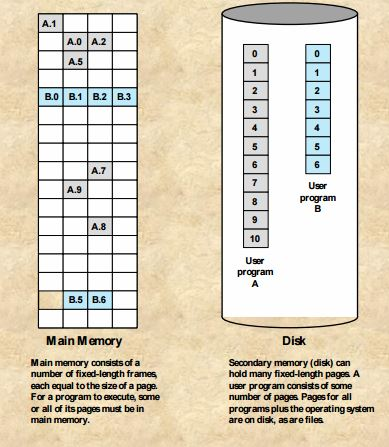
\includegraphics{img/Dynamic_memory.JPG}

\section{Cache Memory \& Operasjon på Stack}
Ved alle instuksjoner så aksesseres minne ved minst en anledning for å hente instruksjonen. Vanligvis flere ganger. Hastigheten som prosessoren kan utføre instuksjoner er åpenbart begrenset av minnets aksesseringstid. Prosessoren har i alle år hatt en mye raskere hastighet enn aksessering av minne. Løsningen har derfor vært å tilegne en liten superrask minne mellom prosessoren og hovedminne, som vi kaller cache. 

\subsection{Cache Principle}
Målet er å tilby markedets raskeste minne, samtidig som den støtter langt billigere minne med mye mer kapasitet. 
\href{http://www.1024cores.net/\_/rsrc/1296469855892/home/parallel-computing/cache-oblivious-algorithms/cpu\_cache\_structure.png}{Konseptet vises i dette bilde}. 
Oppbygningen av Hovedminne består av $2^n$ adresserbare ord (words), der hvert ord har en unik n-bit adresse. Se figur \ref{fig:mem_block}. For "mapping" formål, annser man at minne består av et antall "blocks" med K "words" hver. Det vil si at det er $ M= 2^n/K$ "blocks". Cache Består av C \emph{slots} (også kalt lines) med K words i hver, antallet slots er vesentlig mindre enn antall blocks i hovedminne \emph{( C << M)}. Derfor finner du noen, (ikke alle) subset "blocks" fra hovedminne i cache. Lagt inn som en full linje i cache serielt bortover (ikke parallet nedover som i hovedminne). 

\begin{figure}[h]
\centering
\includegraphics{img/"Cache and main memory block".JPG}
\caption{Cache and main memory block}
\label{fig:mem_block}
\end{figure}

(to be continued, page 52 Stallings).
I arbeid med cache har vi seks temaer som er viktig for designet.
\begin{itemize}
\item Cache Size
\item Block Size 
\item Mapping function 
\item Replacement algorithm 
\item Write policy
\item Number of cache levels 
\end{itemize}
Vi har allerede snakket om "Cache size", det viser seg at en liten cache kan ha en stor påvirkning på "performance". Et annet tema er "block size", mengden data som utveksles mellom cache og hovedminne. Mens "block size" øker fra veldig lite, til større, så vil "hit ratioen" først øke på grunn av principle of locality. Dvs Sannsynligheten for at data i et tidligere refferert "word" blir refferert igjen i nær framtid. Mens "block size" øker enda mer, så vil sannsynligheten for at ...continued.

\subsection{Multiprocessor}
Vanligvis har folk sett på pcen som en sekvensiell maskin som gjør en instruksjon av gangen. Dette er ikke helt sannheten, vi har lenge kjørt pipelining, samtidige kontrollsignaler, og multiprosessering.
Her er de to viktige temaen fra Stallings.
\begin{itemize}
\item Symetric multiprocessors
\item Multicore Computers
\end{itemize}
\subsubsection{Symetric Multiprocessing (SMP)}
En SMP kan defineres som en standalone datamaskin med følgende karakteristikk.
\begin{itemize}
\item Det er to eller flere lignende prosessorer med sammenlignbar kapasitet.
\item Prosessorene deler samme hovedminne, og I/O faseliteter, minneakksessering er relativt likt ved at de er koblet inn på samme bus.
\item Deler I/O devices
\item Alle prosessorene kan utføre samme funksjon (symetric).
\item Systemet kontrolleres av et integrert operativsystem, som tilbyr interragering mellom prosessorene og programmene, ved jobbene(job, task, file, og data element levels).
\end{itemize}

Vi har potensielle fordeler ved SMP.
\begin{itemize}
\item \emph{Performance: }Hvis arbeidet som skal gjøres kan struktureres i parallel så kan vi få en mye bedre ytelse enn ved sekvensiell programmering i samme type prosessor. 
\item \emph{Availability: } I en symetrisk multiprosessor, fordi alle prosessorene kan utføre samme funksjoner så vil ikke en feil i en prosessor ødelegge systemet.
\item \emph{Incremental growth: }En bruker kan øke ytelsen til systemet ved å addere en til prosessor. 
\item \emph{Scalability: }Leverandører kan tilby en stor variasjon i produktet, bassert på antall prosessorer som er konfigurert i systemet.\newline\newline
\end{itemize}
Det er viktig å huske at dette er potensialet, ikke garantert. Det er også viktig å huske at dette kapittelet ikke er nødvendigvis det viktigste temaet på eksamen, men la gå. 
Figur \ref{fig:SMP} viser hvordan den generelle SMP er organisert. 
\begin{figure}
\centering
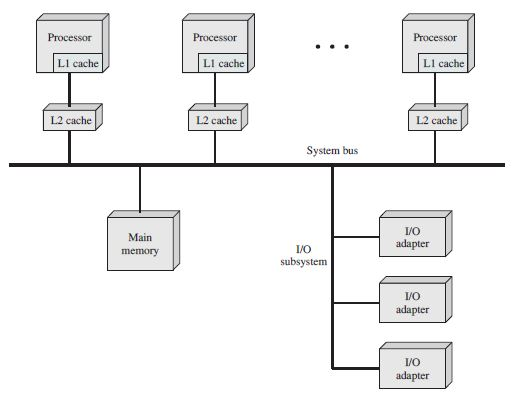
\includegraphics{img/SMP.JPG}
\caption{Symmetric multiprocessing organization}
\label{fig:SMP}
\end{figure}

\subsubsection{Multicore Computers}
Her kombinerer vi to eller flere prosessorer kalt "cores" i en enkel chip (kalt die). Hver "core" har alle komponentene til en singel prosessor, register, ALU, pipeline, L1 instruksjoner og cache. Det er L2 cache og noen ganger L3 cache. Hvis du vil vite hvorfor vi utvikler oss mot denne typen prosessorløsning les boka. 
Se figur \ref{fig:i7} under for oppbygning av Multicore Computers.

\begin{figure}
\centering
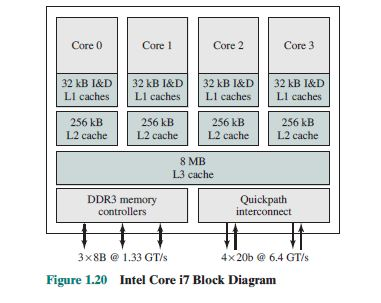
\includegraphics{img/i7.JPG}
\caption{Intel i7 Multicore}
\label{fig:i7}
\end{figure}